\clearpage\newpage
\section{Satisfaction survey}
\label{sec:survey}

This section showcases and analyses the survey made to validate the non-functional requirements.

\subsection{Acquisition}

To get users to answer the survey I've made a popup that shows when the user opens the app and there is at least one subject card in the dashboard. This way we don't ask new users, that wouldn't know what to answer.

In the popup there's a very short text explaining what is the survey for and the estimated time, to motivate users to take it. Below the test there's the answer button and the URL, so they can share it if they want. When the button or the URL are clicked, the \textit{Don't ask again} checkbox is checked.

If the user clicks the \textit{Later} button, the popup closes and it doesn't open again until the user opens the app and one hour has passed. But if he checks the \textit{Don't ask again} checkbox, the button's label changes to \textit{Done}, and the popup will never show again in that device.

\vfill
\begin{figure}[ht!]
    \begin{subfigure}[b]{0.757\textwidth-0.1cm}
        \centering
        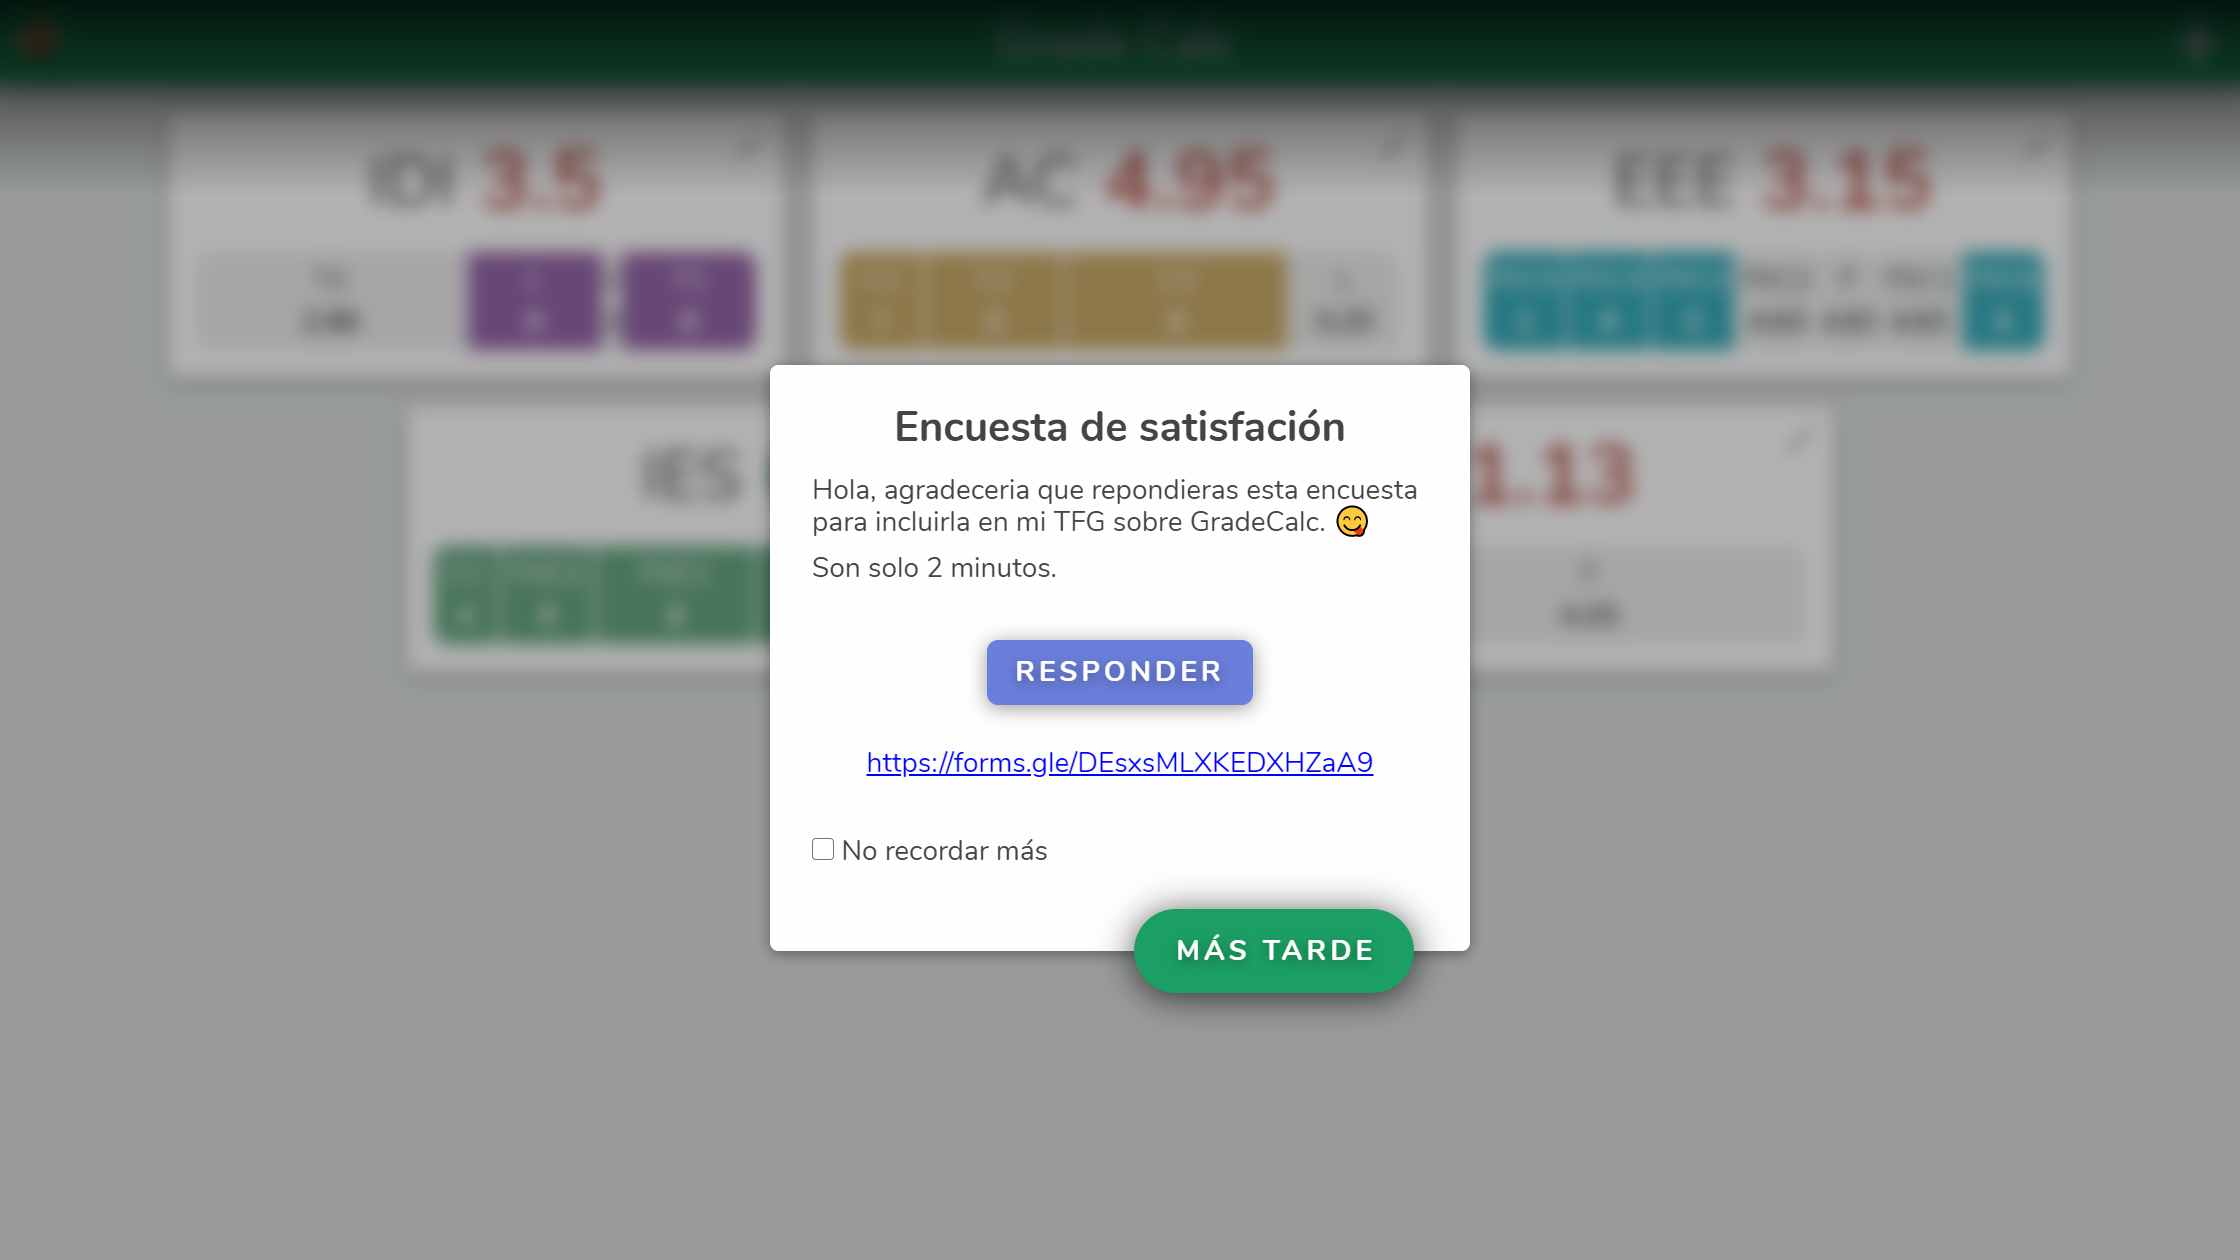
\includegraphics[width=\textwidth]{media/screenshots/screenshot-survey-pc.png}
        \caption{Desktop version}
    \end{subfigure}
    \hfill
    \begin{subfigure}[b]{0.243\textwidth-0.1cm}
        \centering
        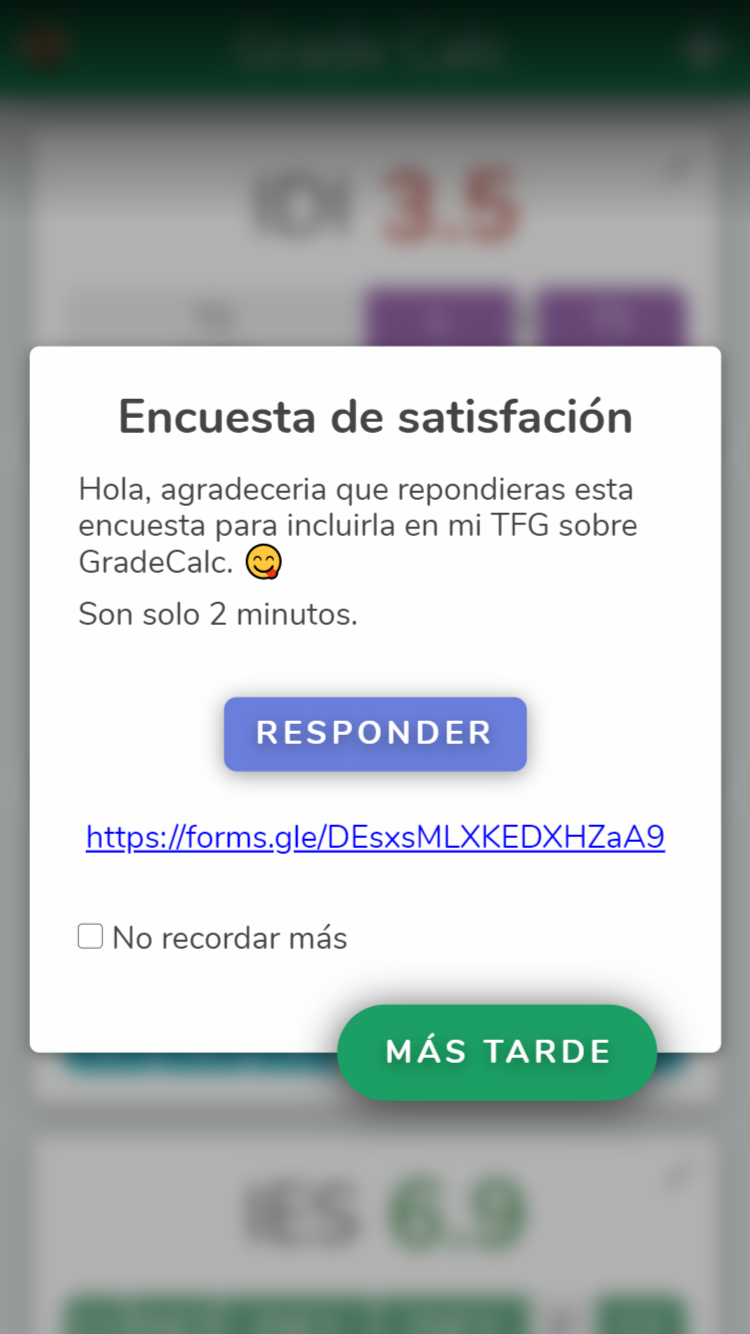
\includegraphics[width=\textwidth]{media/screenshots/screenshot-survey.png}
        \caption{Mobile version}
    \end{subfigure}
    \caption{Satisfaction survey popup}
    \label{fig:screenshot-survey-popup}
\end{figure}
\vfill

The survey is done through Google Forms, and I themed it to match with GradeCalc's aesthetics. It's split up in 4 sections: Introduction, Reliable, Easy to use, and Engaging.

The survey was available for 4 days and 69 users answered it. During this period of time, 321 users opened the app, and 60 of those where new users, so these 60 weren't prompted to take the survey. So 69/261 or 26.4\%, of the prompted users answered the survey.

\vfill
\begin{figure}[h!]
    \center
    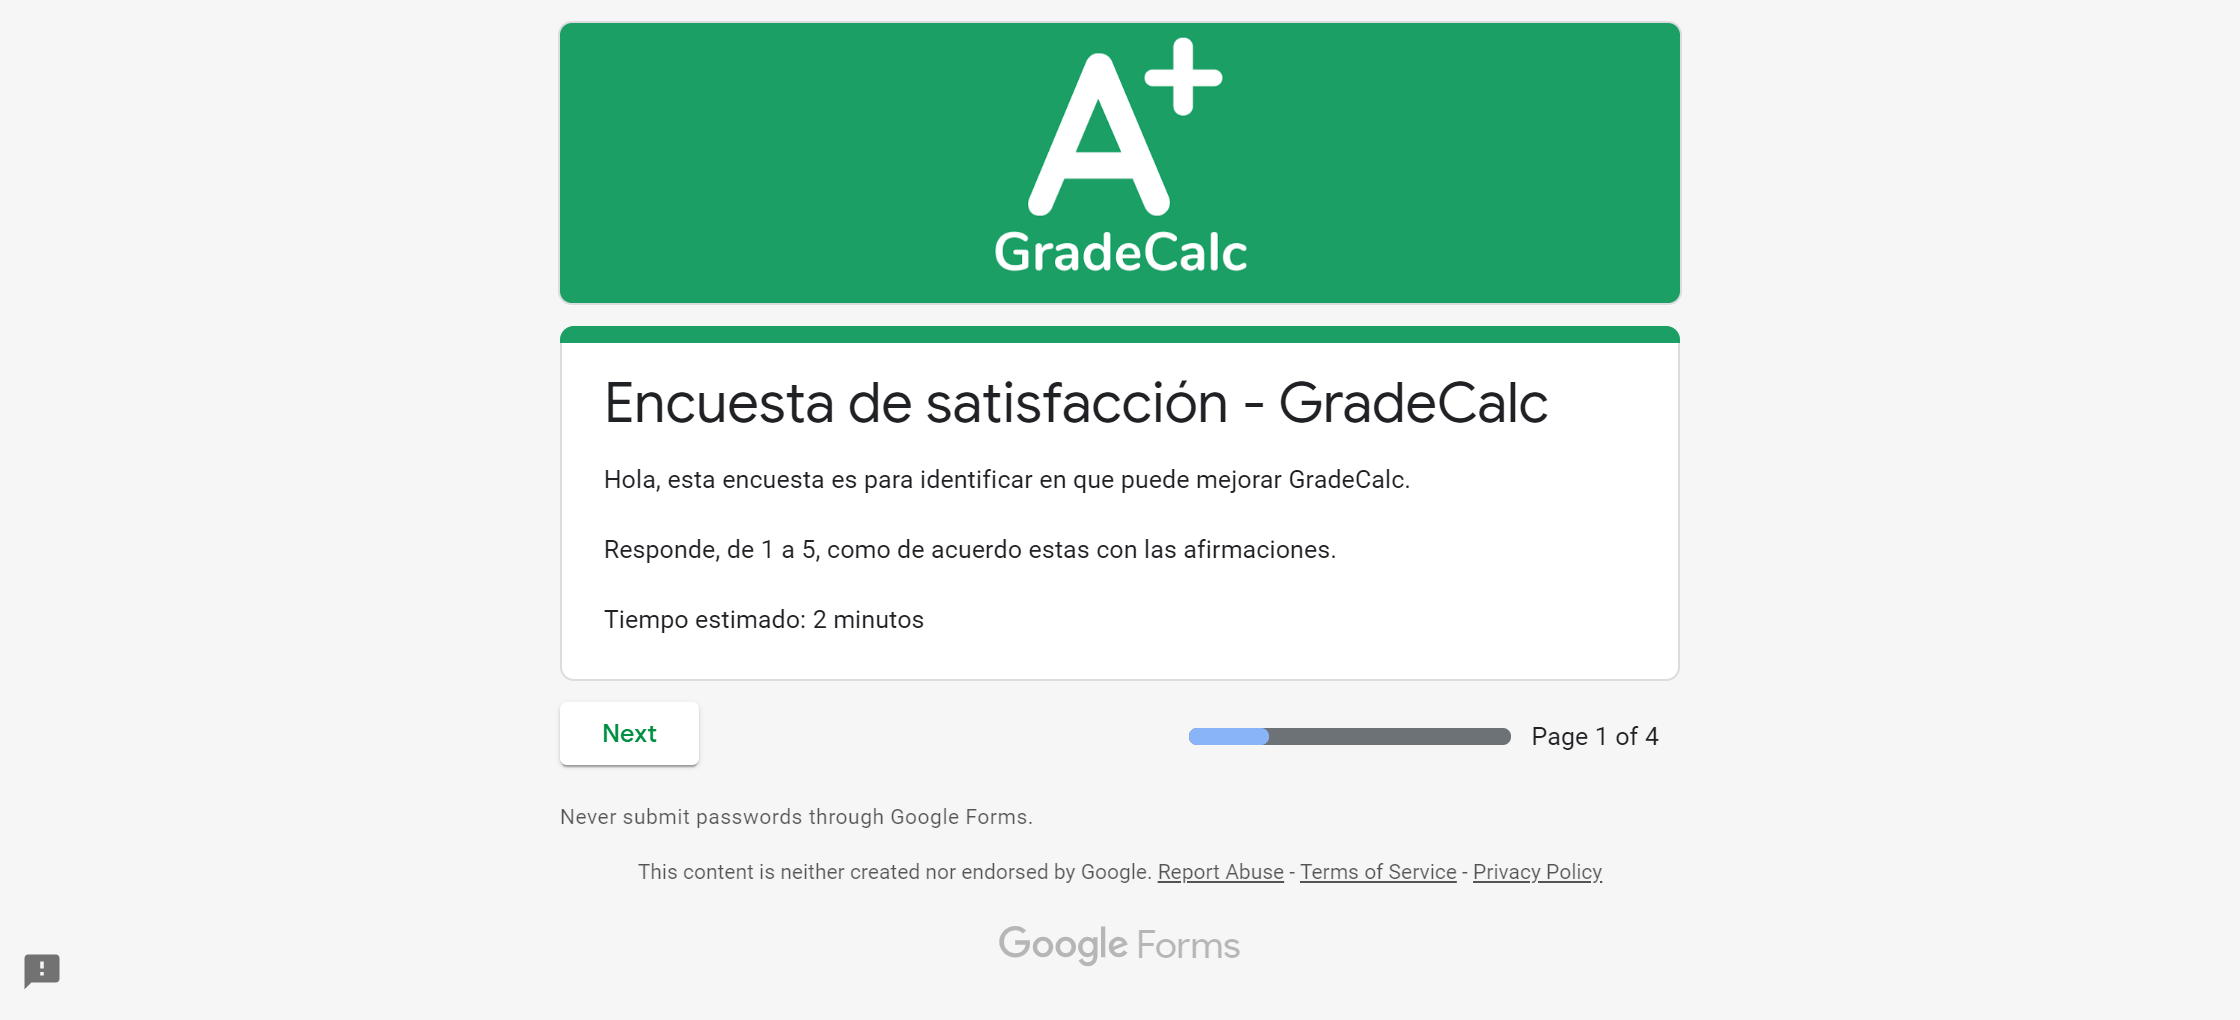
\includegraphics[width=1\columnwidth]{media/survey.png}
    \caption{Satisfaction survey - Introduction}
    \label{fig:screenshot-survey}
\end{figure}
\vfill
\begin{figure}[h!]
    \center
    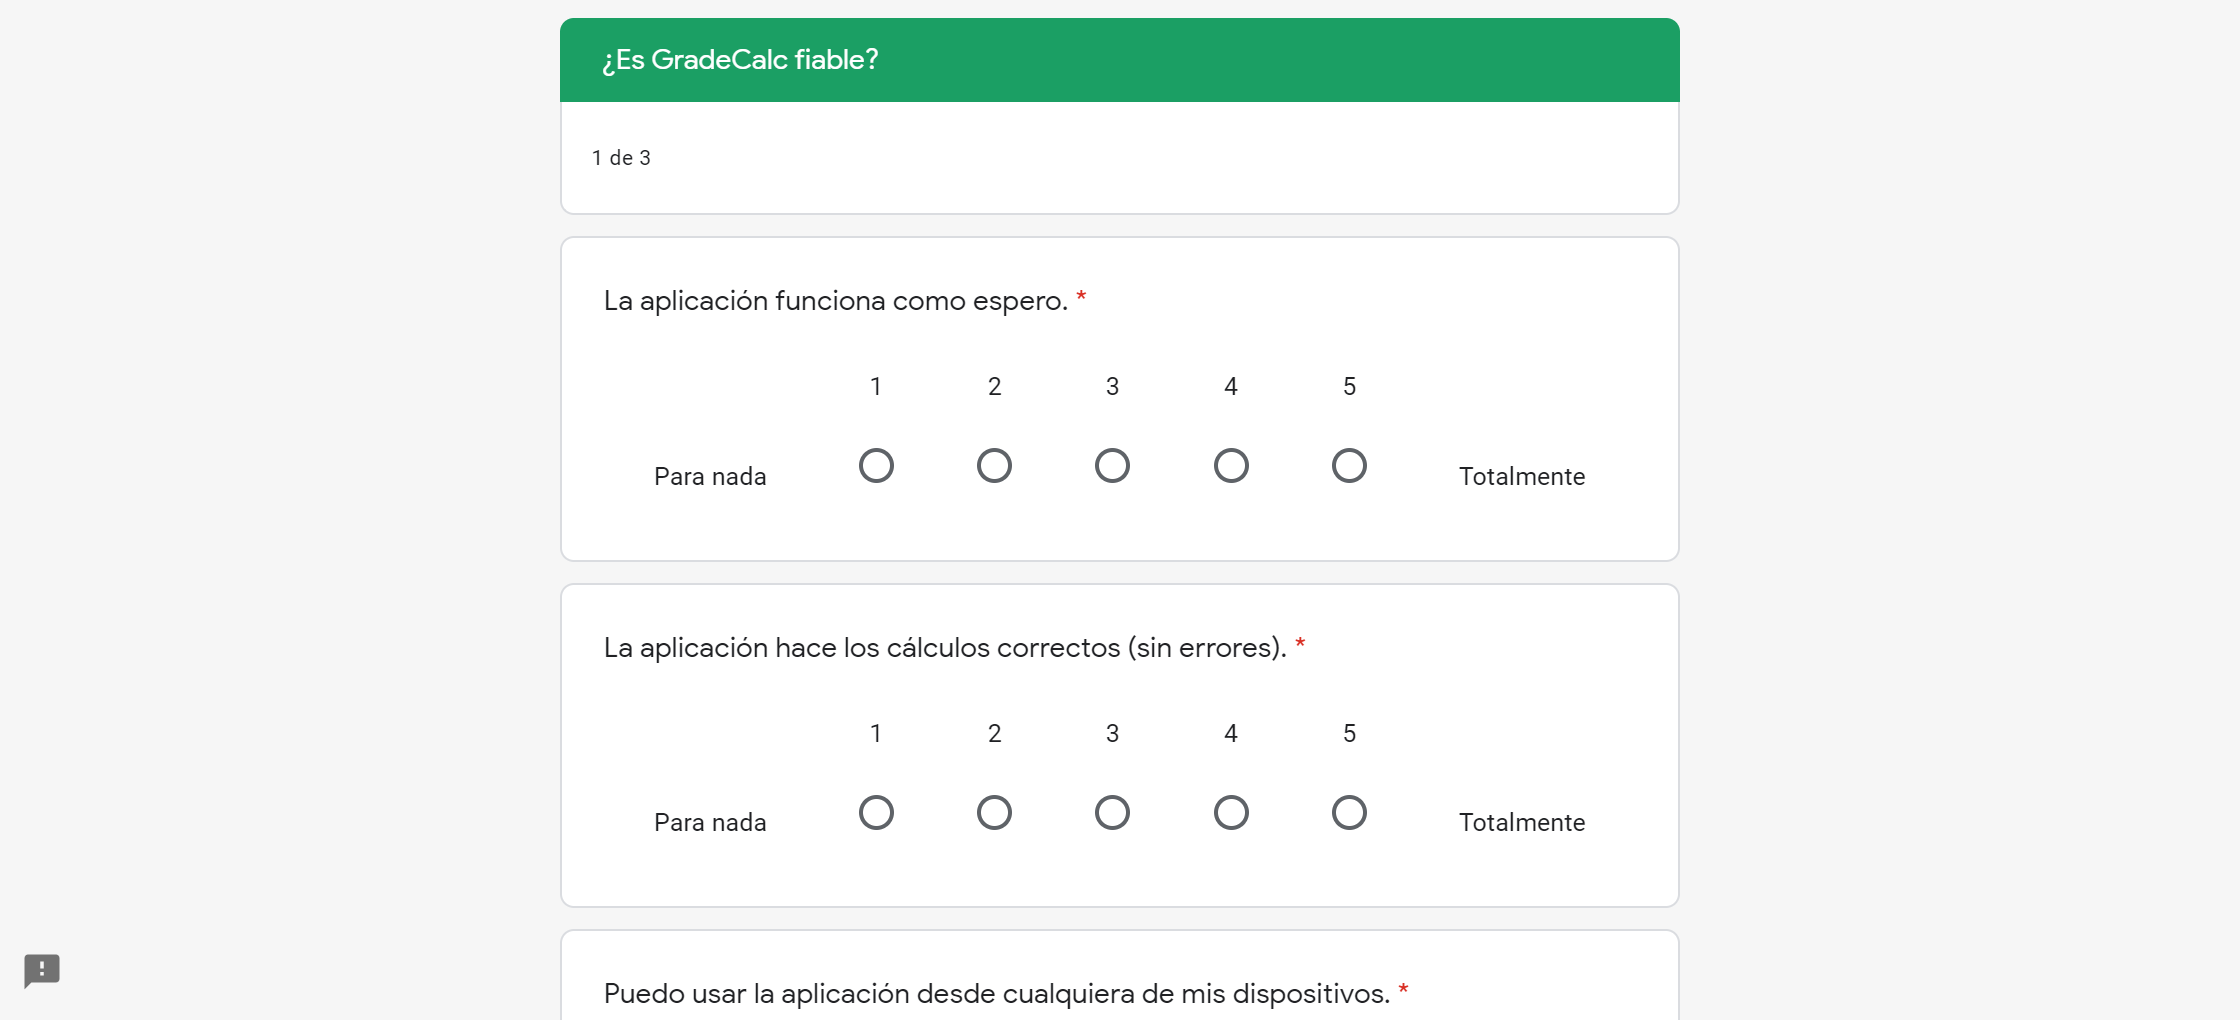
\includegraphics[width=1\columnwidth]{media/survey-2.png}
    \caption{Satisfaction survey - Section 1}
    \label{fig:screenshot-survey-2}
\end{figure}
\vfill

\clearpage\newpage
\subsection{Questions}
The questions made in the survey are the ones formulated to validate the non-functional requirements in section \ref{sec:non-functional}. Users are asked to answer from 1 to 5 how much they agree to the statements. Additionally, there's an extra open question to let users give any feedback they want. These are the statements in Spanish:

% \begin{enumerate}[noitemsep,topsep=0pt]
\begin{enumerate}[noitemsep]
  \item La aplicación funciona como espero.
  \item La aplicación hace los cálculos correctos (sin errores).
  \item Puedo usar la aplicación desde cualquiera de mis dispositivos.
  \item La aplicación guarda mis datos. (Nunca ha perdido datos)
  \item Puedo usar la aplicación para las asignaturas que curso.
  \item La aplicación es fácil de aprender.
  \item La aplicación es fácil de usar.
  \item La aplicación responde rápidamente a mis acciones.
  \item Sé cómo usar la aplicación en general.
  \item Sé cómo crear una asignatura.
  \item Entiendo toda la información de las tarjetas de las  asignaturas.
  \item Disfruto usando la aplicación.
  \item Recomendaría la aplicación.
  \item Hay personas que usan la aplicación gracias a mí.
  \item La aplicación me ayuda a lograr mis objetivos. (En relación con la gestión de tus notas)
  \item La aplicación me ayuda a aprobar las asignaturas.
  \item Abro la aplicación con frecuencia.
  \item Abro la aplicación cuando recibo una nueva nota.
  \item El logo, nombre y estilo de GradeCalc son fáciles de recordar.
  \item Me gustan el logo, nombre y estilo de GradeCalc.
  \item Si quieres, puedes dejar un comentario sobre cualquier otro aspecto de la app. % (Errores, sugerencias...)
\end{enumerate}










\newcommand{\surveyPlot}[2]{
\begin{subfigure}[t]{0.5\textwidth-0.1cm}
    \centering
    
    \begin{tikzpicture}[scale=0.85]
        \begin{axis}[
            ybar, 
            ymin=0,
            % nodes near coords={\pgfmathprintnumber\pgfplotspointmeta\%}
            % nodes near coords={\pgfmathfloatifflags{\pgfplotspointmeta}{0}{}{\pgfmathprintnumber{\pgfplotspointmeta}}}
        ]
            \addplot +[
                hist={data min=1, data max=5},
                % fill=gray!25,
                fill=ForestGreen!33,
                draw=black,
            ] table [y index=#1, col sep=comma, ignore chars="] {media/data/survey.csv};
        \end{axis}
    \end{tikzpicture}
    \caption*{#1. #2}\label{fig:question-plot-#1}
\end{subfigure}
}



\subsection{Answers}
69 users took the survey, these are their answers in the form of plots. All the answers are in the \cref{apx:survey-table} in the form of a table.

\vfill
\begin{figure}[H]
  \surveyPlot{1}{La aplicación funciona como espero.}
  \hfill
  \surveyPlot{2}{La aplicación hace los cálculos correctos (sin errores).}
\end{figure}
\vfill
\begin{figure}[H]
  \surveyPlot{3}{Puedo usar la aplicación desde cualquiera de mis dispositivos.}
  \hfill
  \surveyPlot{4}{La aplicación guarda mis datos. (Nunca ha perdido datos)}
\end{figure}
\vfill
\clearpage\newpage
\vfill
\begin{figure}[H]
  \surveyPlot{5}{Puedo usar la aplicación para las asignaturas que curso.}
  \hfill
  \surveyPlot{6}{La aplicación es fácil de aprender.}
\end{figure}
\vfill
\begin{figure}[H]
  \surveyPlot{7}{La aplicación es fácil de usar.}
  \hfill
  \surveyPlot{8}{La aplicación responde rápidamente a mis acciones.}
\end{figure}
\vfill
\begin{figure}[H]
  \surveyPlot{9}{Sé cómo usar la aplicación en general.}
  \hfill
  \surveyPlot{10}{Sé cómo crear una asignatura.}
\end{figure}
\vfill
\begin{figure}[H]
  \surveyPlot{11}{Entiendo toda la información de las tarjetas de las  asignaturas.}
  \hfill
  \surveyPlot{12}{Disfruto usando la aplicación.}
\end{figure}
\vfill
\begin{figure}[H]
  \surveyPlot{13}{Recomendaría la aplicación.}
  \hfill
  \surveyPlot{14}{Hay personas que usan la aplicación gracias a mí.}
\end{figure}
\vfill
\begin{figure}[H]
  \surveyPlot{15}{{\small La aplicación me ayuda a lograr mis objetivos. (En relación con la gestión de tus notas)}}
  \hfill
  \surveyPlot{16}{La aplicación me ayuda a aprobar las asignaturas.}
\end{figure}
\vfill
\begin{figure}[H]
  \surveyPlot{17}{Abro la aplicación con frecuencia.}
  \hfill
  \surveyPlot{18}{Abro la aplicación cuando recibo una nueva nota.}
\end{figure}
\begin{figure}[H]
  \surveyPlot{19}{El logo, nombre y estilo de GradeCalc son fáciles de recordar.}
  \hfill
  \surveyPlot{20}{Me gustan el logo, nombre y estilo de GradeCalc.}
\end{figure}

\subsubsection*{21. Si quieres, puedes dejar un comentario sobre cualquier otro aspecto de la app. (Errores, sugerencias...)}

\begin{itemize}
  \item Sinceramente, es genial
  \item A veces me resulta confuso el logo porque se parece al de spreadsheets de google. La aplicación es genial y funciona muy bien. Ojalá poder hacer proyectos así algún día.
  \item Podrias hacer una app de android/ios
  \item Sois muy grandes, aplicación súper útil!!!!
  \item Me gustarian mas colores para las diferentes asignaturas, para que no se repitan
  \item Crear asignaturas sin cuenta google
  \item Me gustaría poder reordenar las asignaturas (por ejemplo, arrastrando las tarjetas) y ajustar el tamaño de la cuadrícula en ordenador (poder tener 4 asignaturas en una fila, en una cuadrícula 2x2, etc. Actualmente te obliga a tener filas de 3 asignaturas). También he tenido problemas de pérdida de datos cuando uso la cuenta de google para sincronizar dispositivos. Cuando estén solucionados volveré a usar la app también en el móvil. A parte de esos puntos, es muy buena app y muy útil. No he encontrado ninguna otra que funcione así de bien.
  \item Hay veces que sin querer pongo una nota que no es razonable, como un 70 o algo así, y me sale como asignatura aprobada hasta que borro la nota. Estaría bien que avisara de que la nota no es válida
  \item el único error me aparece al usar la misma cuenta en distintos dispositivos. en ese caso, me aparecen asignaturas duplicadas con distintas notas
  \item Errores al conectarlo con el móvil. Respecto al resto, muy útil.
  \item En algunos dispositivos se queda atascado al crear una asignatura, y no se puede añadir.
  \item No soy ningún experto, y la app es la ostia, pero creo que hay lugar para pequeñas mejoras en UX(/UI).
  \item Hace poco me fallo con el calculo de las assigs pk cambié el \% de los exámenes y proyectos y en próximas veces no lo tenía guardado con el valor que puse yo, sino con el original.
  \item A veces el metodo de avaluacion ha cambiado en la asignatura pero no se ha actualizado en grade calc. Aun así es más que comprensible ya que hay muchas asignaturas y posiblemente muy poca gente gestionando la aplicacion
  \item la parte en la que la gente no suele estar conforme es porque a veces no está actualizado respecto a los cambios en como se evalua la nota de una asignatura. pero todo es fijarse. Es normal que no se pueda estar en todos lados. Por eso siempre hay que ver como son los porcentajes
  \item Plantillas de asignaturas ""oficiales"", a veces para la misma asignatura hay 4 opciones con valores distintos
  \item La aplicación en general está genial y la uso prácticamente a diario o para actualizar cuando hay notas nuevas pero probé a iniciar sesión para que se guardasen mis notas y actualmente la uso sin iniciar sesión porque cuando lo hacía las asignaturas me desaparecían, algunas notas se modificaban o borraban y los campos se ponían aleatoriamente desordenados cada vez que entraba o refrescaba página. Excepto por esos errores la página sin iniciar sesión me ha funcionado siempre perfectamente.
  \item No he encontrado la app en play store y no puedo tener mis notas en el mobil. Cuando abro la web desde el chrome de mi móbil, no se me sincronizan las notas de mi cuenta. Por lo demás es una app maravillosa! 
\end{itemize}





\clearpage\newpage
\subsection{Conclusions}

This is a classification of the questions according to their results.

\begin{itemize}
    \item \textbf{Excellent}: 
        \hyperref[fig:question-plot-2]{2}, 
        \hyperref[fig:question-plot-5]{5}, 
        \hyperref[fig:question-plot-6]{6}, 
        \hyperref[fig:question-plot-7]{7}, 
        \hyperref[fig:question-plot-9]{9}, 
        \hyperref[fig:question-plot-10]{10}, 
        \hyperref[fig:question-plot-11]{11}, 
        \hyperref[fig:question-plot-13]{13}, 
        \hyperref[fig:question-plot-15]{15}, and
        \hyperref[fig:question-plot-18]{18}.
    \item \textbf{Good}: 
        \hyperref[fig:question-plot-1]{1}, 
        \hyperref[fig:question-plot-8]{8}, 
        \hyperref[fig:question-plot-12]{12}, 
        \hyperref[fig:question-plot-14]{14}, 
        \hyperref[fig:question-plot-17]{17}, 
        \hyperref[fig:question-plot-19]{19}, and 
        \hyperref[fig:question-plot-20]{20}.
    \item \textbf{Regular}:
        \hyperref[fig:question-plot-3]{3}, and 
        \hyperref[fig:question-plot-4]{4}.
    \item \textbf{Bad}: 
        \hyperref[fig:question-plot-16]{16}.
\end{itemize}

\noindent
Before proceeding, I have to point out some aspects that may make this survey biased, but are consciously accepted because they still provide relevant feedback. 
\begin{itemize}[noitemsep]
    \item The survey was available for 4 days, so the users that answered the survey are likely to be frequent users, thous more satisfied. The results may be more positive because many non-frequent users didn't participate in it.
    \item The question \hyperref[fig:question-plot-4]{4}, has the word \textit{never}, and this may make the users take the question more strictly, unlike the other ones.
    \item Most questions ask for the user's subjective perception that may not match the reality, For example, in question \hyperref[fig:question-plot-11]{11}, if a user thinks that knows everything shown on the subject card, it doesn't really mean that he knows everything.
    % \item In the question \hyperref[fig:question-plot-17]{17}, different users may understand \textit{frequently} differently. But precision is not relevant in this question, so it's okay.
\end{itemize}

\subsubsection{Excellent}

These are the question where almost all answers are 5 out of 5. From the results, we can conclude that:
\begin{itemize}[noitemsep]
    \item \hyperref[fig:question-plot-2]{2}. 
        The app doesn't miscalculate.
    \item \hyperref[fig:question-plot-5]{5}. 
        The app is suitable for all the user's subjects. 
    \item \hyperref[fig:question-plot-6]{6}. 
        The app is easy to learn.
    \item \hyperref[fig:question-plot-7]{7}. 
        The app is easy to use.
    \item \hyperref[fig:question-plot-9]{9}. 
        Users know how to use the app in general.
    \item \hyperref[fig:question-plot-10]{10}. 
        Users know how to create subjects. This surprised me, I thought that it would score worse.
    \item \hyperref[fig:question-plot-11]{11}. 
        Users understand everything in the dashboard.
    \item \hyperref[fig:question-plot-13]{13}. 
        Users would recommend the app.
    \item \hyperref[fig:question-plot-15]{15}. 
        The app gives users what they want.
    \item \hyperref[fig:question-plot-18]{18}. 
        Users open the app to input their grades when they got new ones, almost always. This means that they have a consistent reason to come back to the app.
\end{itemize}

\noindent
These results are very positive. Most of the questions are excellent, meaning that the users are very satisfied with the app.

\subsubsection{Good}

These are the question where most of the answers are 5 out of 5, but not all. From the results, we can conclude that:

\begin{itemize}[noitemsep]
    \item \hyperref[fig:question-plot-1]{1}. 
        The app mainly works as expected, but 1 third of the users probably are missing a few functionalities. But none thinks that the app is unpredictable.
    \item \hyperref[fig:question-plot-8]{8}. 
        The app is fast, but some users feel that sometimes it could be faster. Everyone agrees the app is not slow.
    \item \hyperref[fig:question-plot-12]{12}. 
        Most of the users enjoy using the app, and I guess that the rest like the app, but isn't very into it. This indicates that GradeCalc adds value to users. 
    \item \hyperref[fig:question-plot-14]{14}. 
        This result is amazing. It means that a large part of GradeCalc's users is promoting the app selflessly. This is the best marketing that the app can have, and also denotes that the users are very satisfied with the app.
    \item \hyperref[fig:question-plot-17]{17}. 
        Most of the users open the app frequently, in their opinion. So, they consider that they don't have the app forgotten.
    \item \hyperref[fig:question-plot-19]{19}. 
        They consider that the brand is easy to remember, but not everyone agrees. 
    \item \hyperref[fig:question-plot-20]{20}. 
        Most of the user's like the branding, many don't care, and none dislikes it.
\end{itemize}

\noindent
These results are also very positive. We see that many aspects work successfully but there's room for improvement.

\subsubsection{Regular}

These are the question that had more bad feedback in relative terms, but still, most of the answers were 5 out of 5. From the results, we can conclude that:
\begin{itemize}[noitemsep]
    \item \hyperref[fig:question-plot-3]{3}. 
        Most of the users can use the app in all their devices, but there's a group that can't. I should investigate what divide is not compatible. But I'd bet that those ones are iPhones and iPads because iOS safari is not optimized for web apps. More research and work needs to be done to improve this score.
    \item \hyperref[fig:question-plot-4]{4}. 
        Most of the users never had any data loss, but there's a group that did. Regarding the ones that lost data, I guess from their answers, that what they lost wasn't a big deal, so this issue doesn't look critical right now. Reading the comments from question \hyperref[fig:question-plot-21]{21}, it appears to be a bug in the synchronization of the grades with the account. More research needs to be done to identify when and what data is lost.
        % My intuition suggests that data losses can happen when users input grades while the app offline, thus they can't be uploaded to their account, and when they go back online, their local data is overwritten by the one in their account. But this is not certain, it's just a guess.
\end{itemize}

\subsubsection{Bad}

\begin{itemize}[noitemsep]
    \item \hyperref[fig:question-plot-16]{16}. 
        This question got a bad scoring, but it's not negative. This question was to know whether users consider that the app helps them to pass subjects or not. Apparently, many people consider that it does, which is great. And many consider that the app has nothing to do with actually passing or not, which also makes sense. I, personally, was expecting that it wouldn't affect.
\end{itemize}

\noindent
We can conclude that there isn't any main issue. At least not present in the survey. 

\subsubsection{The open-ended question}

In the open-ended question \hyperref[fig:question-plot-21]{21}, we can see many positive messages, which is very rewarding as the creator of the app.

Users mainly suggest quality of life features, little changes instead of big changes to the app. I'll note down those suggestions and implement them at some point in the future.
